\documentclass[11pt]{article}
\usepackage{amssymb}
\usepackage{amsmath}
\usepackage{mathrsfs}
\usepackage{bbm}
\usepackage{tikz}
\usepackage{accents}
\usepackage[utf8]{inputenc}
\usepackage[english]{babel}
\usepackage{graphicx}
\usepackage{float}
\usepackage{centernot}
\newcommand{\bs}{{\bigskip}}
\newcommand{\floor}[1]{\lfloor #1 \rfloor}
\newcommand{\ceiling}[1]{\lceil #1 \rceil}
\newcommand{\ms}{{\medskip}}
\newcommand{\sms}{{\smallskip}}
\newcommand{\N}{\mathbb{N}}
\renewcommand{\baselinestretch}{1.2}
\newcommand{\indi}{\mathbbm{1}}
\newcommand{\R}{\mathbb{R}}
\newcommand{\sigF}{\mathcal{F}}
\newcommand{\Z}{\mathbb{Z}}
\newcommand{\C}{\mathbb{C}}
\newcommand{\Q}{\mathbb{Q}}
\newcommand{\E}{\mathbb{E}}
\newcommand{\B}{\mathbb{B}}
\newcommand{\dd}[2]{\frac{d{#1}}{d{#2}}}
\newcommand{\fancyF}{\mathscr{F}}
\newcommand{\borelB}{\mathcal{B}}
\newcommand{\Var}{\text{Var}}
\newcommand{\inner}[2]{\langle{#1},{#2}\rangle}
\newcommand{\sinner}[1]{\langle{#1},{#1} \rangle}
\renewcommand{\epsilon}{\varepsilon}
\renewcommand{\overrightarrow}{\vec}
\newcommand{\tb}{\textbf}
\newcommand{\bfrac}[2]{\displaystyle{\frac{#1}{#2}}}
\newcommand{\bcup}{\bigcup\limits}
\newcommand{\bcap}{\bigcap\limits}
\newcommand{\ceil}[1]{\left\lceil #1 \right\rceil}
\newcommand{\nimply}{\centernot\Rightarrow}
\newcommand{\ar}{\Rightarrow}
\newcommand{\norm}[2]{\| #1 \|_{#2}}
\newcommand{\bnorm}[1]{\norm{#1}{}}
\newcommand{\probp}{\mathbb{P}}
\newcommand{\enorm}[1]{\| #1 \|}
\newcommand{\goto}{\rightarrow}
\newcommand{\bint}[2]{\displaystyle{\int_{#1}^{#2}}}
\newcommand{\nogoto}{\centernot\rightarrow}
\renewcommand{\baselinestretch}{1.2}
\newcommand{\bsum}[2]{\displaystyle{\sum_{#1}^{#2}}}
\newcommand{\bprod}[2]{\displaystyle{\prod_{#1}^{#2}}}
\newcommand{\func}[3]{#1: #2\rightarrow#3}
\newcommand{\sfunc}[2]{#1: #2\rightarrow#2}
\newcommand{\cexp}[2]{\E[#1 \mid #2]}
\usepackage{venndiagram}
\newcommand{\Lim}[1]{\raisebox{0.5ex}{\scalebox{0.8}{$\displaystyle \lim_{#1}\;$}}}
\newcommand{\Limn}{\Lim{n \in \N}}
\newcommand{\Cross}{\mathbin{\tikz [x=1.4ex,y=1.4ex,line width=.2ex] \draw (0,0) -- (1,1) (0,1) -- (1,0);}}
\title{ Transport research notes}
\author{Alois D'uston,  ald6fd}
\setlength{\parindent}{0pt}

\begin{document}


Reference measure $\mu_x \in \probp(\R^d)$,  target measure $\mu_y \in  \probp(\mathcal{M}_y)$.
For 

densities/measures( abuse of notation) $\mu,  \alpha \in \probp(\mathcal{X})$ we define $\alpha \ast \mu$ to be the measure induced by re-sampling random variable $x \sim \mu$ according to $\alpha$. 
The density of $ \alpha \ast \mu$ is just given by product of densities, ie $(\alpha \ast \mu)(x) =  \alpha(x)\mu(x)$.  

Given RKHS $ \mathcal{H}_{\Lambda}$ associated to  PDS kernel $\func{\Lambda}{\mathcal{X} \times \mathcal{X}}{\R}$,  we define
$\probp(\mathcal{H}_{\Lambda}) = \{\alpha(\tilde{x}):= e^{\beta_{\alpha}(\tilde{x})} :  \beta_{\alpha} \in  \mathcal{H}_{\Lambda} \text{ s.t } \int_{\mathcal{X}} e^{\beta_{\alpha}(x)} \: dx = 1  \}$.
Then  for

 $\alpha \in \probp(\mathcal{H}_{\Lambda}) $ we define the enduced 'norm' of $\alpha$ as $\norm{\alpha}{\probp(\mathcal{H}_{\Lambda})} :=  \norm{\beta_{\alpha}}{\mathcal{H}_{\Lambda}} $.

Let $T \in \mathcal{H}_{\Lambda^D}$,   $\alpha_y, \alpha_x \in \probp(\mathcal{H}_{\Lambda})$.  We want to solve for the 'optimal' latent 

re-sampling of $\mu_y$.   By optimal we mean 

I.  There exists a good( in MMD sense) and regular( in $\norm{\cdot}{\mathcal{H}_{\Lambda^D}}$ sense) transport map $T$ from $\mu_x$ to $\alpha_y \ast \mu_y$.

II.  There exists a good( in MMD sense) and regular( in $\norm{\cdot}{\mathcal{H}_{\Lambda}}$ sense) 

resampling map  $\alpha_x$ from  $\alpha_y \ast \mu_y$ to $\mu_y$.   

We obtain this map as the solution to the following optimization problem.
$$\alpha_y^* = \underset{\alpha_y, \alpha_x,  T}{\text{argmin}} \text{ MMD}(\alpha_x \ast T^{\#}\mu_x,  \mu_y)\: + \text{MMD}(T^{\#}\mu_x,  \alpha_y \ast			\mu_y) +\lambda_1\norm{T}{H_T}  + \lambda_2\norm{\alpha_y}{\probp(\mathcal{H}_{\Lambda})}$$

This optimization problem admits representor form  in terms of 
$Z \in \R^{n \times D}$,  

$ \beta_Y, \beta_X   \in \{ \beta \in \R^n:  \norm{\exp(\beta)}{1} = 1\}$ and $\alpha_Y,  \alpha_X := \exp(\beta_Y),   \exp(\beta_X)$.

\sms

 $\alpha_Y^* = \underset{\alpha_Y,   \alpha_X,  Z}{\text{argmin }}  \hat{\text{MMD}}(\alpha_X,  Z) + \hat{\text{MMD}}(\alpha_Y,  Z)  + \norm{\hat{Z}}{\mathcal{H}_\Lambda} + \norm{\hat{\alpha_Y}}{\probp(\mathcal{H}_{\Lambda})} $  for

\sms

I.  $\hat{\text{MMD}}(\alpha_X,  Z)  =  \alpha_X^T K(Z,Z)\alpha_X^T -\frac{2}{n} \alpha_X^TK(Z,Y)\indi$

II.  $\hat{\text{MMD}}(\alpha_Y,  Z)  =   \alpha_Y^T K(Y,Y)\alpha_Y - \frac{2}{n}\indi^TK(Z,Y)\alpha_Y$


III.  $\norm{\hat{Z}}{H_\Lambda} = \text{ trace}(Z^T\Lambda(X,X)^{-1}Z)$,
IV.  ${\norm{\hat{\alpha_Y}}{\probp(\mathcal{H}_{\Lambda})}} =
\beta_Y^T\Lambda(Y,Y)^{-1}\beta_Y $



In practice can use correction factors and add penalty losses to ensure $\norm{\exp(\beta_X)}{1},\norm{\exp(\beta_Y)}{1} \approx 1$.  I've found emperically this works fairly well.


The idea here is that  this optimization  yields a $T^{\#}\mu_x$ which is a good a proxy for some 
latent resampling 
 of $\mu_y$, 
   ie 
$T^{\#}\mu_x \sim \alpha_y \ast \mu_y$ and $\alpha_x = \alpha_y^{-1}$.

Further by including RKHS norms we ensure $T^{\#},  \alpha_y$ are regular.  

We cannot regularize $\alpha_x$ directly as it's domain is  the support of $\alpha_y \ast \mu_y$ and not or $\mu_x$ or $\mu_y$.  However,  note $\alpha_x = \alpha_y^{-1}$,  and resampling maps have the special property that 
$\beta_{\alpha_y^{-1}}= - \beta_{\alpha_y}$.  I have  strong intuition that in this case regularizing $\alpha_y$ will be equivalent to regularzing $ \alpha_y^{-1} = \alpha_x$. The numerical experiments I've so far agree with this,  though a proof is beyond me so far



\pagebreak




Regularity of $\alpha_Y$ is $\underset{\mu_y^N}{\E}[{\norm{\hat{\alpha_Y}}{\probp(\mathcal{H}_{\Lambda})}}] = \underset{Y \sim \mu_y^N}{\E}[\beta_{\alpha_y}(Y)^T\Lambda(Y,Y)^{-1}\beta_{\alpha_y}(Y)]$


\ms


Regularity of $\alpha_Y^{-1}$ is 
$\underset{ \alpha_Y \ast \mu_y}{\E}[{\norm{\hat{\alpha_Y^{-1}}}{\probp(\mathcal{H}_{\Lambda})}}] = \underset{\tilde{Y}  \sim (\alpha_Y \ast \mu_y)^N}{\E}[\beta_{\alpha_y^{-1}}(Y)^T\Lambda(\tilde{Y},\tilde{Y})^{-1}\beta_{\alpha_y^{-1}}(Y)]$

\ms

Some numerical tests I did to this effect:

\bs


 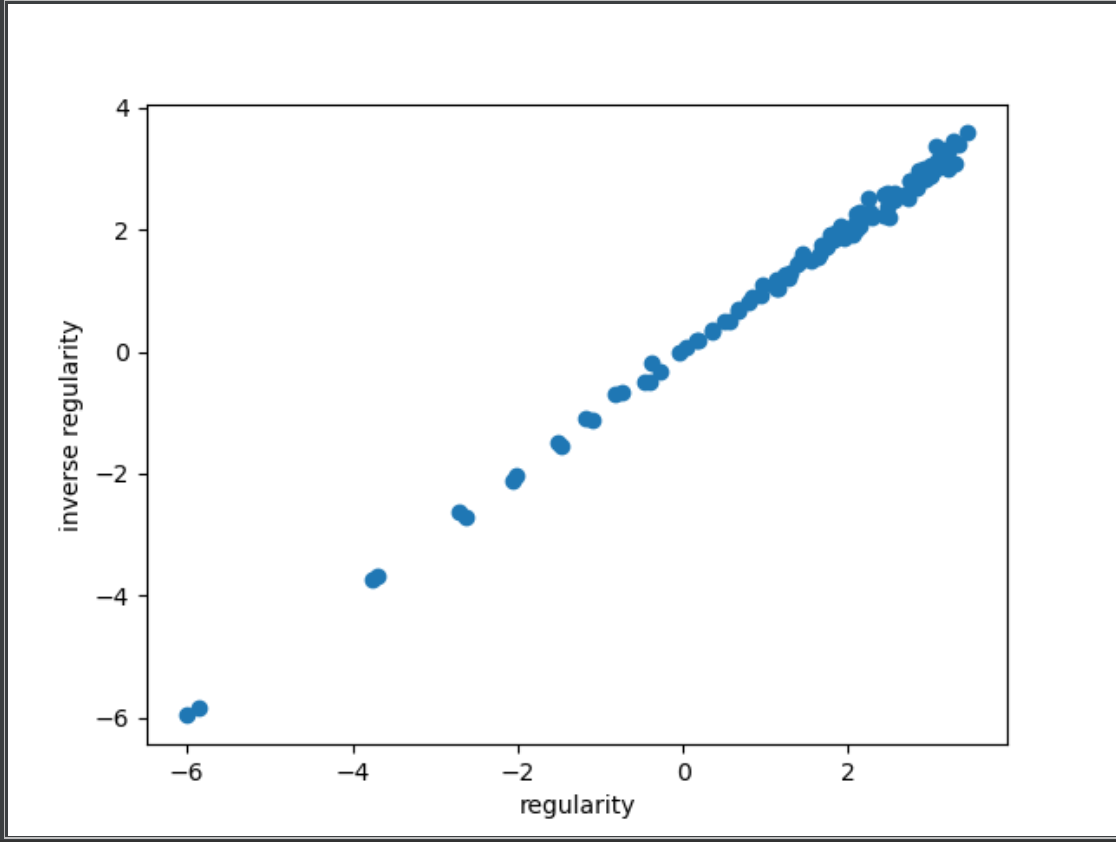
\includegraphics[width=100mm]{reg_comparison.png}




\pagebreak


\end{document}
